%% 
%% Copyright 2007-2019 Elsevier Ltd
%% 
%% This file is part of the 'Elsarticle Bundle'.
%% ---------------------------------------------
%% 
%% It may be distributed under the conditions of the LaTeX Project Public
%% License, either version 1.2 of this license or (at your option) any
%% later version.  The latest version of this license is in
%%    http://www.latex-project.org/lppl.txt
%% and version 1.2 or later is part of all distributions of LaTeX
%% version 1999/12/01 or later.
%% 
%% The list of all files belonging to the 'Elsarticle Bundle' is
%% given in the file `manifest.txt'.
%% 
%% Template article for Elsevier's document class `elsarticle'
%% with harvard style bibliographic references

%% \documentclass[preprint,12pt,authoryear]{elsarticle}

%% Use the option review to obtain double line spacing
%% \documentclass[authoryear,preprint,review,10pt]{elsarticle}

%% Use the options 1p,twocolumn; 3p; 3p,twocolumn; 5p; or 5p,twocolumn
%% for a journal layout:
%% \documentclass[final,1p,times,authoryear]{elsarticle}
%% \documentclass[final,1p,times,twocolumn,authoryear]{elsarticle}
%% \documentclass[final,3p,times,authoryear]{elsarticle}
%% \documentclass[final,3p,times,twocolumn,authoryear]{elsarticle}
%% \documentclass[final,5p,times,authoryear]{elsarticle}
\documentclass[final,5p,times,twocolumn,authoryear]{elsarticle}

%% For including figures, graphicx.sty has been loaded in
%% elsarticle.cls. If you prefer to use the old commands
%% please give \usepackage{epsfig}

%% The amssymb package provides various useful mathematical symbols
\usepackage{amssymb}
%% The amsthm package provides extended theorem environments
%% \usepackage{amsthm}

%% The lineno packages adds line numbers. Start line numbering with
%% \begin{linenumbers}, end it with \end{linenumbers}. Or switch it on
%% for the whole article with \linenumbers.
%% \usepackage{lineno}

% ggpackages
\usepackage{amsmath}
\usepackage{amsfonts}       % blackboard math symbols
\usepackage{algorithm}      % http://ctan.org/pkg/algorithms
\usepackage{algpseudocode}  % http://ctan.org/pkg/algorithmicx
\usepackage{nicefrac}       % compact symbols for 1/2, etc.
\usepackage{graphicx}
\usepackage[font=small,skip=0pt]{subcaption}  % subcaption automatically loads caption package
\usepackage{booktabs}       % professional-quality tables
\usepackage{hyperref}       % hyperlinks
\usepackage{url}            % simple URL typesetting
\usepackage{rotating}       % sidewaystable
\usepackage[utf8]{inputenc}       % sidewaystable
\usepackage[dvipsnames]{xcolor}   % \textcolor{red}{il mio testo}
\usepackage{soul}  % highlight
% \usepackage{xcolor}

\newcommand{\figref}[1]{Fig.~\ref{#1}}
\newcommand{\figrefp}[1]{(\figref{#1})}
\newcommand{\tabref}[1]{Tab.~\ref{#1}}
\newcommand{\tabrefp}[1]{(\tabref{#1})}
\newcommand{\eqnref}[1]{Eq.~(\ref{#1})}

\newcommand{\tbc}[0]{\textbf{> > > TO BE CHECKED < < <}}
\newcommand{\tbm}[0]{\textbf{> > > TO BE MODIFIED < < <}}
\newcommand{\tbe}[0]{\textbf{> > > TO BE EXPANDED < < <}}

\newcommand{\cf}[0]{\textit{cf. }}
\newcommand{\eg}[0]{\textit{e.g., }}
\newcommand{\ibid}[0]{\textit{ibid.}}
\newcommand{\ie}[0]{\textit{i.e.,}}
\newcommand{\etc}[0]{\textit{etc.}}

\newcommand{\supmat}[0]{\hyperref[sec:supmat]{\textit{Supplementary Material}} }
\newcommand{\asupmat}[0]{\hyperref[sec:supmat]{\textit{Sup. Mat.}} }

% Abbreviations
\newcommand{\rhs}[0]{right hand side}  % right hand side
\newcommand{\lhs}[0]{left hand side}  % left hand side
\newcommand{\snr}[0]{snr}  % signal-to-noise ratio
% Definitions
\newcommand{\realnumbers}[0]{\mathbb{R}}
\newcommand{\norm}[1]{\left\lVert#1\right\rVert}
% boldface symbols
\newcommand{\ab}[0]{\mathbf{a}}
\newcommand{\bb}[0]{\mathbf{b}}
\newcommand{\xb}[0]{\mathbf{x}}
\newcommand{\setx}[0]{\mathbf{x}_1,\ldots,\mathbf{x}_C}
\newcommand{\setxn}[0]{\mathbf{x}_1^{(n)},\ldots,\mathbf{x}_C^{(n)}}
\newcommand{\yb}[0]{\mathbf{y}}
\newcommand{\zb}[0]{\mathbf{z}}
\newcommand{\dz}[0]{d\zb}
% colored symbols
\newcommand{\xc}[0]{\color{blue}x\color{black}}
\newcommand{\xbc}[0]{\color{blue}\xb\color{black}}
\newcommand{\yc}[0]{\color{olive}y\color{black}}
\newcommand{\ybc}[0]{\color{olive}\yb\color{black}}
% bold symbols
\newcommand{\alphab}[0]{\boldsymbol{\alpha}}
\newcommand{\thetab}[0]{\boldsymbol{\theta}}
\newcommand{\thetaset}[0]{\thetab_1,\ldots,\thetab_C}
\newcommand{\phib}[0]{\boldsymbol{\phi}}
\newcommand{\phiset}[0]{\phib_1,\ldots,\phib_C}
\newcommand{\etab}[0]{\boldsymbol{\eta}}
\newcommand{\epsilonb}[0]{\boldsymbol{\epsilon}}
\newcommand{\x}[0]{\xb}
\newcommand{\xdn}[0]{\xb_{d,n}}
\newcommand{\xdnv}[0]{\xb_{d,n,v}}
\newcommand{\xdnw}[0]{\xb_{d,n,w}}
\newcommand{\z}[0]{\zb}
\newcommand{\Lin}[0]{\mathbf{L}}
\newcommand{\mub}[0]{\boldsymbol{\mu}}
\newcommand{\Sigmab}[0]{\boldsymbol{\Sigma}}
\newcommand{\sigmab}[0]{\boldsymbol{\sigma}}
% cal symbols
\newcommand{\Dcal}[0]{\mathcal{D}}
\newcommand{\Lcal}[0]{\mathcal{L}}
\newcommand{\Qcal}[0]{\mathcal{Q}}
% Gaussian
\newcommand{\Gauss}[2]{\mathcal{N}\left(#1;#2\right)}
\newcommand{\Gaussof}[1]{\mathcal{N}\left(#1\right)}
\newcommand{\Gausstd}[0]{\Gauss{\mathbf{0}}{\mathbf{I}}}
\newcommand{\GaussStdDim}[1]{\Gauss{\mathbf{0}}{\mathbf{I}_{#1}}}
% Kullback-Leibler
\newcommand{\kl}[0]{\operatorname{\mathcal{D}_{KL}}}
\newcommand{\KL}[2]{\kl\left(#1||#2\right)}
% Expected Value
\newcommand{\expect}{\operatorname{\mathbb{E}}}
\newcommand{\Var}{\operatorname{Var}}
\newcommand{\Cov}{\operatorname{Cov}}
\newcommand{\VAR}[1]{\Var\left[#1\right]}
\newcommand{\COV}[1]{\Cov\left[#1\right]}
\newcommand{\E}[1]{\expect\left[#1\right]}
\newcommand{\EE}[2]{\expect_{#1}\left[#2\right]}
% Marginal / Joint probabilities
\newcommand{\q}[1]{q\left(#1\right)}
\newcommand{\p}[1]{p\left(#1\right)}
\newcommand{\px}[0]{\p{\x}}
\newcommand{\pz}[0]{\p{\z}}
\newcommand{\pxz}[0]{\p{\x,\z}}
\newcommand{\psetx}[0]{\p{\setx}}
\newcommand{\psetxz}[0]{\p{\setx,\z}}
% Conditional probabilities
\newcommand{\pxgz}[0]{\p{\x|\z}} % x Given z
\newcommand{\psetxgz}[0]{\p{\setx|\z}}
\newcommand{\pzgsetx}[0]{\p{\z|\setx}}
\newcommand{\pzgx}[0]{\p{\z|\x}}
% Posterior
\newcommand{\pzsetx}[0]{\p{\z|\setx}}
% Variational approximation
\newcommand{\qz}[0]{\q{\z}}
\newcommand{\qzgx}[0]{\q{\z|\x}}
\newcommand{\qzgsetx}[0]{\q{\z|\setx}}
\newcommand{\qzg}[1]{\q{\z|#1}}
\newcommand{\qzx}[1]{\q{\z|\x_{#1}}}
% Lower Bound
\newcommand{\lb}[0]{\mathcal{L}}
\newcommand{\LBdnv}[0]{\lb_v^{(\xdn)}}
\newcommand{\LBdnvw}[0]{\lb_{v \leftarrow w}^{(\xdn)}}
\newcommand{\LBof}[1]{\lb\left( #1 \right)}
\newcommand{\LBn}[0]{\LBof{\xdnv}}
\newcommand{\LB}[0]{\LBof{\mathcal{D}}}
% EXPECTATION PROPAGATION
\newcommand{\qi}[0]{q_i(\thetab)}
\newcommand{\qj}[0]{q_j(\thetab)}
\newcommand{\cavity}[0]{Q_{\backslash i}(\thetab)}
% Sets
\newcommand{\set}[1]{\left\{#1\right\}}
% Optimization
\newcommand{\argmin}{\operatorname{arg\,min}}
\newcommand{\argmax}{\operatorname{arg\,max}}
\newcommand{\optim}{\operatorname{Optim}}


\journal{Neuroimage}

\begin{document}

\begin{frontmatter}

%% Title, authors and addresses

%% use the tnoteref command within \title for footnotes;
%% use the tnotetext command for theassociated footnote;
%% use the fnref command within \author or \address for footnotes;
%% use the fntext command for theassociated footnote;
%% use the corref command within \author for corresponding author footnotes;
%% use the cortext command for theassociated footnote;
%% use the ead command for the email address,
%% and the form \ead[url] for the home page:
%% \title{Title\tnoteref{label1}}
%% \tnotetext[label1]{}
%% \author{Name\corref{cor1}\fnref{label2}}
%% \fntext[label2]{}
%% \cortext[cor1]{}
%% \address{Address\fnref{label3}}
%% \fntext[label3]{}

\title{
% Multi-Task Learning from Datasets with Missing Observations:
% Application to Multi-Modal Neuroimaging Studies in Dementia
Combining Multi-Task Learning and Multi-Channel Variational Auto-Encoders to Exploit Datasets with Missing Observations -
Application to Multi-Modal Neuroimaging Studies in Dementia
}
%% 
%% %% use optional labels to link authors explicitly to addresses:
%% %% \author[label1,label2]{}
%% %% \address[label1]{}
%% %% \address[label2]{}
%% 
%% \author{
%% 	L. Antelmi,
%% 	N. Ayache,
%% 	P. Robert,
%% 	M. Lorenzi,\\
%% 	for the Alzheimer's Disease Neuroimaging Initiative.
%% }
%% 
%% \address{}

\author{Luigi Antelmi \fnref{epione}\corref{luigi}}
\author{Nicholas Ayache \fnref{epione}}
\author{Philippe Robert\fnref{cobtex,cmrr}}
%
\author{Federica Ribaldi\fnref{lane,unibs,lanvie,memoryclinic}}
\author{Valentina Garibotto\fnref{garibotto1,garibotto2}}
\author{Giovanni B. Frisoni\fnref{lanvie,memoryclinic}}
%
\author{Marco Lorenzi\fnref{epione}}
%
\author{for the Alzheimer's Disease Neuroimaging Initiative \corref{adni}}

\fntext[epione]{University of Côte d'Azur, Inria, Epione Project-Team, France.}
\fntext[cobtex]{University of Côte d'Azur, CoBTeK, France.}
\fntext[cmrr]{Centre Mémoire, CHU of Nice, France}
%
\fntext[lane]{Laboratory of Alzheimer’s Neuroimaging and Epidemiology (LANE), Saint John of God Clinical Research Centre, Brescia, Italy.}
\fntext[unibs]{Department of Molecular and Translational Medicine, University of Brescia, Brescia, Italy.}
\fntext[lanvie]{Laboratory of Neuroimaging of Aging (LANVIE), University of Geneva, Geneva, Switzerland.}
\fntext[memoryclinic]{Memory Clinic, Geneva University Hospitals, Geneva, Switzerland.}
\fntext[garibotto1]{Laboratory of Neuroimaging and Innovative Molecular Tracers (NIMTlab), Geneva University Neurocenter and Faculty of Medicine, University of Geneva, Geneva, Switzerland.}
\fntext[garibotto2]{Division of Nuclear Medicine and Molecular Imaging, Diagnostic Department, Geneva University Hospitals, Geneva, Switzerland.}
%
\cortext[luigi]{Corresponding author: luigi.antelmi@inria.fr}
\cortext[adni]{
Data used in preparation of this article were obtained from the Alzheimer's Disease Neuroimaging Initiative (ADNI) database (http://adni.loni.usc.edu).
As such, the investigators within the ADNI contributed to the design and implementation of ADNI and/or provided data but did not participate in analysis or writing of this report.
A complete listing of ADNI investigators can be found at 
http://adni.loni.usc.edu/wp-content/uploads/how\_to\_apply/ADNI\_Acknowledgement\_List.pdf
}

\begin{abstract}
% The abstract should briefly summarize the contents of the paper in
% 150--250 words.
% \keywords{First keyword  \and Second keyword \and Another keyword.}
The joint modeling of different biomedical datasets requires the ability of consistently analyzing heterogeneous information in presence of often non-overlapping sets of views, or modalities (e.g. clinical scores, imaging data, or biological measurements), which may be missing for economical, ethical, or scarcity reasons.
This problem requires to deal with random and non-random missing data specific to each dataset, under the form of missing measurements corresponding to a given view.
%
We propose here a generative latent-variable model of the common variability across datasets, based on the estimation of a shared latent representation across views.
Our formulation allows to retrieve a consistent latent representation common to all data-types and datasets, even if datasets share only partially overlapping subsets of views.
%
Experiments on synthetic data show that our method is able to identify a common latent representation of multi-feature datasets, even when the overlap of views in the feature-sets across datasets is minimal.
% The resulting latent representation is generally equivalent to one obtained with a model trained with no missing data-types.
%
When analyzing independent dementia datasets containing heterogeneous clinical and imaging data modalities, our model is able to mitigate the absence of views in datasets.
Moreover, the common latent representation inferred with our model can be used to define robust classification models gathering the combined information across different datasets.

\end{abstract}

% %%Graphical abstract
% \begin{graphicalabstract}
% %\includegraphics{grabs}
% \end{graphicalabstract}

% %%Research highlights
% \begin{highlights}
% \item Research highlight 1
% \item Research highlight 2
% \end{highlights}

% \begin{keyword}
% %% keywords here, in the form: keyword \sep keyword
% 
% %% PACS codes here, in the form: \PACS code \sep code
% 
% %% MSC codes here, in the form: \MSC code \sep code
% %% or \MSC[2008] code \sep code (2000 is the default)
% 
% \end{keyword}

\end{frontmatter}
%% \linenumbers

%% main text
\section{Introduction}

Because of the inherent complexity of biomedical data and diseases,
researchers are required to integrate data across different studies to increase the sample size and obtain better models \citep{LeSueur2020}.
%
In the development of integrative models, researchers have to face with multiple concurrent challenges, such as the ones related to
datasets interoperability \citep{Tognin2020},
data heterogeneity \citep{Buch2020},
and data missingness \citep{GolrizKhatami2020}.
%
Emblematic is the case of integrative modeling when datasets come from multi-centric studies in cognitive and neurological disorders,
such as the Alzheimer's Disease (AD).
%
Here the datasets interoperability is hampered by the existence of different protocols between studies.
Because of this, methods whose modeling task are specifically designed on one dataset cannot be directly applied to another dataset.
%
Furthermore, at the level of each single dataset researchers face the challenge of modeling heterogeneous data,
such as multiple imaging modalities, clinical scores and biological measurements.
Because each one of these sources of information represents an important and independent \textit{view} on the disease or phenomena under investigation,
efforts to model multi-view data are ubiquitous in the recent literature \citep{Vieira2020}, where the objective ranges from predicting clinical outcomes \citep{Chen2019} to synthesizing new modalities \citep{Zhou2020, Wei2019}.
%
Another common problem to the joint modeling of multiple datasets is represented by missing data.
At the level of the single datasets, views can be missing at random (MAR) for some subjects.
Typically, as fitting multi-view models requires to establish connections between views, observations with at least one missing view are totally discarded, yielding to potentially severe loss of available information.
To mitigate this problem, imputation methods are usually applied to infer missing views by modeling the relationship across views from complete observations.
% As an example, $k$-Nearest Neighbor is a popular approach based on the imputation from $k$ nearest neighbors found in the observations with full views.
%
The loss of information is exacerbated when considering multiple datasets altogether.
Indeed, according to the cohort study design, there may be views which are specifically absent, hence missing not at random (MNAR).
This potential mismatch across datasets hampers their interoperability,
and prevents the gathering of all the available observations into a single, robust and generalizable joint model accounting for the global data variability.
%
% This challenge is typically addressed in machine learning by the fields of Transfer Learning (TL) and Multi Task Learning (MTL).
% TL is based on the transfer of model parameters across datasets \citep{TL}.
% This paradigm is commonly applied to datasets with compatible modalities (e.g. from image to image) and in its basic form consists in using the parameters trained on the first dataset to initialize the training on a second dataset.
% Unfortunately, this often leads to the problem known as catastrophic forgetting \citep{CatastroficForgetting}, consisting of neural networks that loose the information learned from the first modeling task after training a second one.
%
This challenge is typically addressed in machine learning by the field of Multi Task Learning (MTL).
To address this issue, MTL aims at improving the model interoperative capabilities by exploiting the information extracted from multiple datasets.
In MTL each task is usually associated to the modeling of a specific dataset and its views only,
and the main idea is to share across datasets the parameters learned through each modeling task \citep{Caruana1998, Dorado-Moreno2020}.
As an example of MTL, in model-agnostic meta-learning (MAML) \citep{MAML1} the training of a model on a variety of learning tasks enforces the generalization on new datasets after few fine tuning iterations.
As a result this model can solve new learning tasks after few re-training epochs.
Nevertheless, these approaches present scalability issues, as for example MAML requires the costly computation of Hessian vectors across dataset parameters.
%
In the context of neural networks, MTL is usually achieved with specific output layers for every task, and by including a shared representation for all of them \citep{Dorado-Moreno2020}.
This modeling rationale is at the basis of recent MTL based approaches to heterogeneous data assimilation \citep{Wu2018, Antelmi2019, Shi2019}.
In particular, approaches such as the The Multi-Channel Variational Autoencoder (MCVAE) \citep{Antelmi2019} rely on the identification of a common latent representation for different views belonging to a single dataset.
Training these models is possible with some limitations:
1) after having discarded observations with missing views;
2) when all the training observations are compatible in terms of available views, and hence are usually limited to model one dataset at a time.

To overcome these limitations, here we investigate an extension of MCVAE to simultaneously learn from multiple datasets, even in the presence of non compatible views between datasets, and missing views within datasets.
Our extension \figrefp{fig:model} is build upon the following actions:
1) to regroup all the subjects with compatible views into a new dataset that has no missing views by construction,
2) to associate each one of these newly defined datasets to a specific modeling task,
3) to stack multiple instances of the MCVAE, where each instance models a specific task,
4) share the models parameters of common views between modeling tasks.
%
Thanks to all these actions, our method allows to learn a joint model for all the subjects without discarding any information.
The common views between tasks act as a bridge and enable the information to flow through all the other views.
In the training phase, tasks lacking a particular view will simply not contribute to the learning of those view-specific parameters.
All the tasks will nevertheless benefit from the parameters they didn't contribute to learn, for the prediction of their missing views.
The variational formulation for computing approximate posterior distributions of the latent variables allows fast and scalable training.
Being dataset agnostic, our method allows to integrate all the available data into a joint model, gathering  all the available information from multiple datasets at the same time.

The rest of this paper is structured as follow.
In \S~\ref{sec:method} we set the theoretical framework for our model.
In \S~\ref{sec:synth} experiments on synthetic data show that the prediction error of missing views is competitive with respect to the one obtained with state of the art imputation methods.
In \S~\ref{sec:real} experiments on real data from independent multi-modal neuroimaging datasets show that our model generalizes better than dataset-specific models on new unseen data, in both the tested cases of imaging derived phenotypes auto-encoding and diagnosis classification.
Lastly we discuss our results and limitations and conclude our work with summary remarks.

\section{Method}
\label{sec:method}

In this section we recall the theoretical framework of the \textit{Multi-Channel Variational Autoencoder} (MCVAE) developed in our previous work \citep{Antelmi2019}, which we now extend to tackle the problem of missing data integration.
In \S~\ref{ssec:generative_model} and \S~\ref{ssec:derivation} we introduce the approach and derive the model in presence of missing data.
In \S~\ref{ssec:parameterization} we briefly recall the main parametric functions adopted later in our experiments with missing data.
In \S~\ref{ssec:optimization} we finally propose the new optimization scheme allowing to account for observations with partially missing views.
Code developed in Pytorch \citep{Paszke2019} is publicly available at \url{https://gitlab.inria.fr/epione\_ML/mcvae}.

\subsection{Generative Model}
\label{ssec:generative_model}

Let $\Dcal = \set{D_d}_{d=1}^D$ be a collection of $D$ independent datasets, where each dataset $D_d = \set{\xdn}_{n=1}^{N_d}$ is composed by $N_d$ independent data-points (\eg subjects in the case of medical imaging datasets).
Every dataset $D_d$ is associated with a total number of $V_d$ available views
(\eg sets of clinical scores and imaging derived phenotypes extracted from multiple imaging modalities),
and we assume that each data-point $\xdn = \set{\xdnv}_{v=1}^{V_{d,n}}$ is composed by $V_{d,n}$ views,
where $V_{d,n} \leq V_d$.
With the latest inequality we account for data-points with an arbitrary number of missing views.

For each view $\xdnv$ we rely on the following generative latent variable model:
\begin{equation}\label{eq:model}
\begin{aligned}
&\z_{d,n} \sim \p{\z}, \\  % = \GaussStdDim{l} \\
&\xdnv \sim \p{\xdnv|\z_{d,n},\thetab_v},  % = \Gauss{\mub_c(\z)}{\Sigmab_c(\z) | \thetab_c}
\qquad \textnormal {for} \; v \; \textnormal{in} \; 1 \ldots V_{d,n} \leq V_d,
\end{aligned}
\end{equation}
where $\pz$ is a prior distribution for the latent variable $\z_{d,n}$ commonly shared by the $V_{d,n}$ views, and
where the likelihood functions $\p{\xdnv|\z_{d,n},\thetab_v}$ belong to a family of distributions parametrized by $\thetab_v$, which represents the view-specific generative parameters shared among all datasets.

\subsection{Inference Model}
\label{ssec:derivation}

The exact solution to the inference problem is given by the posterior $\p{\z|\set{\xdnv,\thetab_v}_{v=1}^{V_{d,n}}}$, that is not generally computable analytically.
Following \cite{Antelmi2019}, we can nevertheless look for its approximation through \textit{Variational Inference} \citep{Blei2017}, applied in our specific context of missing data.

The variational approximations $\q{\z|\x_{d,n,w}, \phib_w}$, where $\phib_w$ represents the view-specific variational parameters shared among all datasets, are such that:
%
\begin{equation}\label{eq:newLB}
	\begin{aligned}
		\ln \p{\xdnv|\thetab_v} \geq \LBdnv = \frac{1}{V_{d,n}} \sum_{w=1}^{V_{d,n}} \LBdnvw,
	\end{aligned}
\end{equation}
%
where:
%
\begin{equation}\label{eq:LBdnvw}
	\begin{aligned}
		\LBdnvw = \EE{q_{d,n,w}(\z)}{\ln \p{\xdnv|\z, \thetab_v}} - \KL{q_{d,n,w}(\z)}{\pz}
	\end{aligned}
\end{equation}
%
is the lower bound associated to the data-point $\xdn$ when its view $v$ is predicted from its view $w$.
%
In \figref{fig:architecture} we sketch the model structure induced by \eqnref{eq:LBdnvw}.
The complete derivation of \eqnref{eq:newLB} is detailed in the \supmat\ section of this work.

\begin{figure}[htbp]
\centering
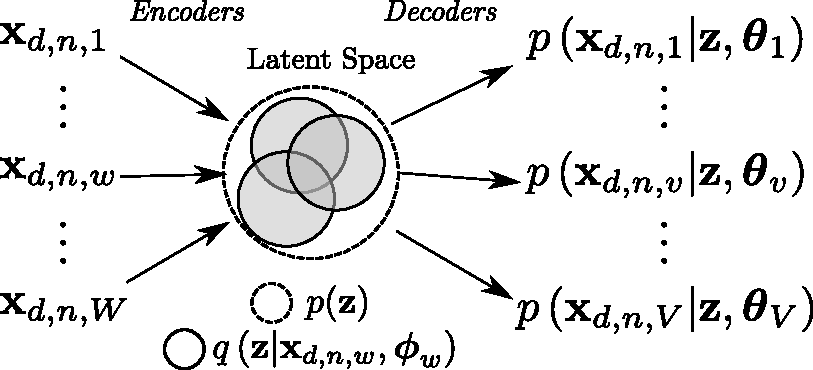
\includegraphics[width=\columnwidth]{./tex/fig/architecture.pdf}
\caption{
General variational framework for our multi-view model.
For every pair of views $v$ and $w$ there is a prediction path $v \leftarrow w$ composed by two learnable functions: the encoding distribution $\q{\z|\xb_w, \phib_w}$ and the decoding likelihood $\p{\xb_v|\z, \thetab_v}$.
Parameters $\phib_w$ and $\thetab_v$ are optimized through \eqnref{eq:argmax} to maximize the likelihood of our generative model under the encoding distributions, and at the same time minimize the Kullback-Leibler distance between every encoder and the prior $\pz$.
To leave the notation uncluttered, in this representation we dropped the dataset index $d$ and data-point $n$ used in the text.
}
\label{fig:architecture}
\end{figure}


\subsection{Optimization}
\label{ssec:optimization}

Assuming independent observations, the marginal log-likelihood in the left hand side of \eqnref{eq:newLB} can be summed up over all the datasets, data-points, and views.
As a consequence, inference on the model generative parameters $\thetab = \set{\thetab_v}$ and variational parameters $\phib = \set{\phib_w}$ can be achieved by solving the maximization problem:
\begin{equation}\label{eq:argmax}
\begin{aligned}
\hat{\thetab}, \hat{\phib} &= \underset{\thetab, \phib}{\argmax} \sum_{d,n,v} \LBdnv \\
                           &= \underset{\thetab, \phib}{\argmax} \sum_{d,n,v} \frac{1}{V_{d,n}} \sum_{w=1}^{V_{d,n}} \LBdnvw.
\end{aligned}
\end{equation}
%
\begin{algorithm} % enter the algorithm environment
\caption{Model parameters optimization} % give the algorithm a caption
\label{alg:optim} % and a label for \ref{} commands later in the document
\begin{algorithmic} % enter the algorithmic environment
	\Require Initialize the model parameters $\phib, \thetab$. Set the optimizer learning rate.
	\While{$\phib, \thetab$ not converged}
		\State $\lb \leftarrow 0$
		\For{every dataset $d \in D$}
			\For{every datapoint $n \in N_d$}
				\For{every \textit{decoding} view $v \in V_{d,n}$}
					\State $\lb_v \leftarrow 0$
					\For{every \textit{encoding} view $w \in V_{d,n}$}
						\State Accumulate the cost of decoding $\xdnv$ through the encoder $q_{d,n,w}(\z)$:
						\State $\lb_v \leftarrow \lb_v + \EE{q_{d,n,w}(\z)}{\ln \p{\xdnv|\z, \thetab_v}} - \KL{q_{d,n,w}(\z)}{\pz}$.
					\EndFor
					\State Average the decoding cost and accumulate it in the total cost $\lb$:
					\State $\lb \leftarrow \lb + \frac{1}{V_{d,n}} \lb_v$.
				\EndFor
			\EndFor
		\EndFor
		\State $\thetab, \phib = \optim(\phib, \thetab, \nabla_{\phib} \lb, \nabla_{\thetab} \lb)$. \textit{Adam} optimizer used to maximie $\lb$.
	\EndWhile
\end{algorithmic}
\end{algorithm}
% \begin{algorithm} % enter the algorithm environment
% \caption{Calculate $y = x^n$} % give the algorithm a caption
% \label{alg1} % and a label for \ref{} commands later in the document
% \begin{algorithmic} % enter the algorithmic environment
%     \REQUIRE $n \geq 0 \vee x \neq 0$
%     \ENSURE $y = x^n$
%     \STATE $y \Leftarrow 1$
%     \IF{$n < 0$}
%         \STATE $X \Leftarrow 1 / x$
%         \STATE $N \Leftarrow -n$
%     \ELSE
%         \STATE $X \Leftarrow x$
%         \STATE $N \Leftarrow n$
%     \ENDIF
%     \WHILE{$N \neq 0$}
%         \IF{$N$ is even}
%             \STATE $X \Leftarrow X \times X$
%             \STATE $N \Leftarrow N / 2$
%         \ELSE[$N$ is odd]
%             \STATE $y \Leftarrow y \times X$
%             \STATE $N \Leftarrow N - 1$
%         \ENDIF
%     \ENDWHILE
% \end{algorithmic}
% \end{algorithm}

%
We implemented Algorithm \ref{alg:optim} to solve \eqnref{eq:argmax}.
The summation in \eqnref{eq:argmax} is done for every dataset $d$ along all the available data-points $n$ and their specific views $v$.
If missing, a particular view $v$ will be simply not accounted for that specific observation, without having to discard all the other views that can still contribute to optimize \eqnref{eq:argmax}.
We note that batching data-points with common views can speed up the computation by reducing the number of second level \textit{for} loop iterations in Algorithm \ref{alg:optim}.
The presence of at least one common view among datasets acts as a link across datasets and allows the information to flow through all the datasets to the other views.
In \figref{fig:model} the learning scheme of our model in a simple case with four views and one common view between batches.

\begin{figure*}[htbp]
\centering
\includegraphics[width=\textwidth]{./tex/fig/model.pdf}
\caption{
Simple example of a Multi-Task Model learning scheme in the presence of missing not available (NA) views.
Arrows represent learnable functions used as network encoders and decoders, transforming respectively input views (\eg clinical scores, imaging derived phenotypes, \ldots) from the observation space to the representation space (circles) and from the representation space back to the observation space.
The separability of the loss function $\LBdnv$ in \eqnref{eq:newLB} allows to group together observations into homogeneous learning tasks.
For every task, functions associated to missing views (dashed gray arrows) are locally not updated by the learning algorithm.
Globally, common latent representations (red circles) across pairs of tasks act as a link allowing the information to flow throughout the views.
}
\label{fig:model}
\end{figure*}


\subsection{Comparison with VAE and MCVAE}
In \tabref{tab:mcvae} we show how our Multi-Task model extends the capabilities of the Multi-Channel VAE (MCVAE, \cite{Antelmi2019}), which is itself a multi-view extension of the VAE \citep{Kingma2013,Rezende2014}.

In our former work we proposed a multi-view generative model trainable only with observation in the training set have all the available views, limited to model one dataset at a time (in the case of datasets with multiple views), after having discarded incomplete observations in that dataset.
We address this limitation by allowing missing views in the training set for some observations, thanks to the adapted optimization scheme in \eqnref{eq:argmax}.
\begin{table}[h]
\centering
\caption{
	The Multi-Task Multi-Channel VAE (MT-MCVAE) extends the MCVAE, which is itself an extension of the VAE.
}
\label{tab:mcvae}
\resizebox{\columnwidth}{!}{
	\begin{tabular}{lccc}
	\toprule
		Method                          &  Train with missing data  &  Test with missing data  &  \# views modeled  \\
	\midrule
		VAE       &  no   &  no   &  $1$   \\
		MCVAE     &  no   &  yes  &  $>1$  \\
		MT-MCVAE  &  yes  &  yes  &  $>1$  \\
	\bottomrule
	\end{tabular}
}
\end{table}


As in the MCVAE, at test time, the trained MT-MCVAE model can estimate missing views $\hat\xb_{d,n,v}$ from the available ones through the formula:
\begin{equation}\label{eq:reconstruction}
\begin{aligned}
\hat\xb_{d,n,v} = \frac{1}{V_{d, n}-1} \sum_{w=1, \,w\neq v}^{V_{d, n}} \EE{q_{d,n,w}(\z)}{\p{\xdnv|\z, \thetab_v}},
\end{aligned}
\end{equation}
where the available views $\xdnw$ are encoded into the distributions $q_{d,n,w}$, which are then used to predict the missing view through its decoding distribution $\p{\xdnv|\z, \thetab_v}$.

\subsection{Parameterization}
\label{ssec:parameterization}

With the right choice of the functional form of $\q{\z|\x_{d,n,w}, \phib_w}$, $\pz$, and $\p{\xdnv|\z, \thetab_v}$, the \rhs\ of \eqnref{eq:newLB} becomes amenable to computation and optimization, yielding to the maximization of the \lhs, quantity also known as the model evidence.
Of course, the choice for the likelihood function $\p{\xdnv|\z, \thetab_v}$ depends on the nature of the view $\xdnv$.
For example it can be parametrized as a multivariate Gaussian in the case of continuous data (\ie imaging derived phenotypes), as a Bernoulli likelihood for dichotomic data, and as a Categorical likelihood for categorical data.

\subsubsection{Linear parameterization}
In general, the prior distribution $\pz$ is the  multivariate Gaussian distribution $\Gausstd$.
The same family of distributions is also commonly used for the variational and likelihood functions, such that respectively:
\begin{alignat}{4}
\label{eq:encoder}
\q{\z|\xdnw, \phib_w}  &= \mathcal{N} \left( \mub = \mathbf{V}_w^{(\mu)} \xdnw \right. &&{}; &&\left.\Sigmab = \diagp{\mathbf{V}_w^{(\sigma)} \xdnw} \right), \\
\label{eq:decoder}
\p{\xdnv|\z,\thetab_v} &= \mathcal{N} \left( \mub = \mathbf{G}_v^{(\mu)} \zb \right. &&{} ; &&\left.\Sigmab = \diagp{\mathbf{g}_v^{(\sigma)}} \right),
\end{alignat}
where the moments $\mub$ and $\Sigmab$ are obtained from linear transformations of the conditioning variables.
Here, $\thetab_v = \{\mathbf{G}_v^{(\mu)}, \mathbf{g}_v^{(\sigma)}\}$ and $\phib_w=\{\mathbf{V}_w^{(\mu)}, \mathbf{V}_w^{(\sigma)}\}$ are the parameters to be optimized.
A non-linear parameterization can be used as well, for example in the form of deep neural networks.

In \cite{Antelmi2019} we also introduced the following alternative parameterization for the posterior distribution:
\begin{equation}
\label{eq:dropout_posterior}
    q_{d,n,w}(\z) = \Gauss{\mub = \mathbf{V}_w^{(\mu)} \xdnw}{\Sigmab = \diagp{\sqrt{\alphab} \odot \mub^2}},
\end{equation}
which is known as \textit{dropout posterior} \citep{Kingma2015}.
The dropout parameter $\alphab$ has components $\alpha_i = \nicefrac{p_i}{1-p_i}$ linked to the probability $p_i$ of dropping out the $i$-th latent variable component \citep{Wang2013}.
It has been shown that the association of this dropout posterior with a log-uniform prior distribution $\pz$ leads to sparse and interpretable models \citep{Antelmi2019,Molchanov2017}.

Thanks to the flexibility of modern neural network frameworks,
it is straight forward to implement non linear parametrizations $\mub = \mathbf{f}^{(\mu)}(\x)$ and $\Sigmab = \mathbf{f}^{(\sigma)}(\x)$ for the mean and covariance functions in the variational and likelihood distributions.
Typically it is done by stacking linear or convolution layers, interleaved with non-linear activation functions such as sigmoid and hyperbolic tangent.

The use of non linear networks can provide better results.
The design choices that the model user must make
(for example the number of layers, the sizes of hidden dimensions, the activation functions, \etc),
is in general highly task-dependent.

\section{Synthetic Experiments}
\label{sec:synth}

In this section we describe our results on extensive synthetic experiments performed with our model and benchmark methods in two conditions:
1) views missing at random for each dataset,
and 2) datasets with systematically missing views (missing not at random).

%%%%%%%%%%%%%%%%%%%%%%%%%%%
%% SYNTHETIC EXPERIMENTS %%
%%%%%%%%%%%%%%%%%%%%%%%%%%%
\subsection{Data preparation}

To simulate multi dataset observations, we sample the latent variable $\z_{d,n}$ from a multivariate Gaussian with zero-mean and identity covariance matrix, and then we transform it with random linear mapping towards the observation space to get $\xdnv$.
We then corrupt the observation with increasing levels of noise
and we apply specific strategies to remove views in the context of the \textit{missing at random} (MAR) and \textit{missing not at random} (MNAR) experiments.

%% MAR %%
In the MAR experiments views were randomly removed according to a parameter $0 \leq f \leq 1$, which controls the fraction of data-points with complete views.
In the extreme case $f=1$, all the data-points have all the views, representing the ideal case of no missing views, that is the working case of the Multi-Channel Variational Autoencoder \citep{Antelmi2019}.
In the case $f=0$, each data-point has one and only one randomly assigned view, representing the case where no relationship between views can be established.
Here our multi-view model collapses to a disjoint series of independent Variational Autoencoders \citep{Kingma2013, Rezende2014}.
In the general case, each data-point has probability $f$ to have all the views, and probability $1-f$ to have a randomly assigned view out of the total available views.
The general case represents the case where the relationship between views can be established only through a fraction $f$ of the total available data-points.

%% MNAR %%
In the MNAR experiments we removed specific views for each simulated dataset, ensuring at the same time the absence of at least one view for a datasets, and the presence of at least one view in common between pairs of datasets.
As an example, in the case with three datasets and three views, the association view-dataset can be expressed through the following association matrix $A$:
\begin{equation}
A = 
\begin{pmatrix}
1 & 0 & 1 \\
1 & 1 & 0 \\
0 & 1 & 1 
\end{pmatrix},
\end{equation}
where $A(v,d)=1$ indicates the presence of view $v$ in dataset $d$.
We limited our MNAR simulations to cases that can be defined with square association matrices having a dimensionality not greater than $5$.

\subsection{Model Fitting and Evaluation}

In both MAR and MNAR experiments we fit the synthetic scenarios with our model, where we choose a linear Gaussian parametrization for the variational and likelihood distributions, such that respectively:
\begin{align}
\label{eq:encoder}
q_{d,n,w}(\z) &= \Gaussof{\mub=\mathbf{V}_w^{(\mu)} \xdnw, \Sigmab = diag(\mathbf{V}_w^{(\sigma)} \xdnw)}, \\
\label{eq:decoder}
\p{\xdnv|\z,\thetab_v} &= \Gaussof{\mub = \mathbf{G}_v^{(\mu)} \zb, \Sigmab = diag(\mathbf{g}_v^{(\sigma)})},
\end{align}
\textit{i.e.} factorized multivariate Gaussian distributions whose moments are linear transformations depending on the conditioning variables. \\
$\thetab_v = \{\mathbf{G}_v^{(\mu)}, \mathbf{g}_v^{(\sigma)}\}$ and $\phib_w=\{\mathbf{V}_w^{(\mu)}, \mathbf{V}_w^{(\sigma)}\}$ are the parameters to be optimized through (\ref{eq:argmax}).
Lastly we predicted for each simulated scenario the missing views according to \eqnref{eq:reconstruction} on testing hold-out datasets.

Results, cross validated $5$ times, were summarized with the \textit{mean squared error} (MSE) metric on testing hold-out datasets for every simulated scenario.
We applied the same evaluation procedure for the following benchmark methods.

\subsection{Benchmark Methods}
Among state of the art multivariate linear and non linear imputation methods, we selected the following competitors as a benchmark:
1) k-Nearest Neighbors (knn) with $k=\set{1, 5}$;
2) Denoising Autoencoder (DAE);
3) Multivariate Imputation by Chained Equations (MICE).

For the knn approach we used the \textit{KNNImputer} method as implemented in the \textit{Scikit-Learn} library \citep{sklearn}.
Here each sample's missing values are imputed using the mean value from $k$ nearest neighbors found in the training set.
Two samples are close if the features that neither is missing are close in terms of Euclidean distance.

The Denoising Autoencoder, as developed by \cite{dae}, is based on an overcomplete deep autoencoder.
It maps input data to a higher dimensional space, which in combination with an initial dropout layer inducing corruption, makes the model robust to missing data.
We used the same architecture proposed by the authors, that is three hidden layers for encoder and decoder networks, Tanh activation functions, hyperparameter $\Theta=7$, and dropout $p=0.5$, as they proved to provide consistent better results.

In MICE, as implemented in \cite{mice}, missing values are modeled as a multivariate linear combination of the available features.
This methodology is attractive if the multivariate distribution is a reasonable description of the data, which in our case it is by construction.
MICE specifies the multivariate imputation model on a variable-by-variable basis by a set of conditional densities, one for each incomplete variable.
Starting from an initial imputation, MICE draws imputations by iterating over the conditional densities.

\subsection{Results}
\begin{figure}[htb]
\centering
\begin{subfigure}{.49\textwidth}
	\centering
        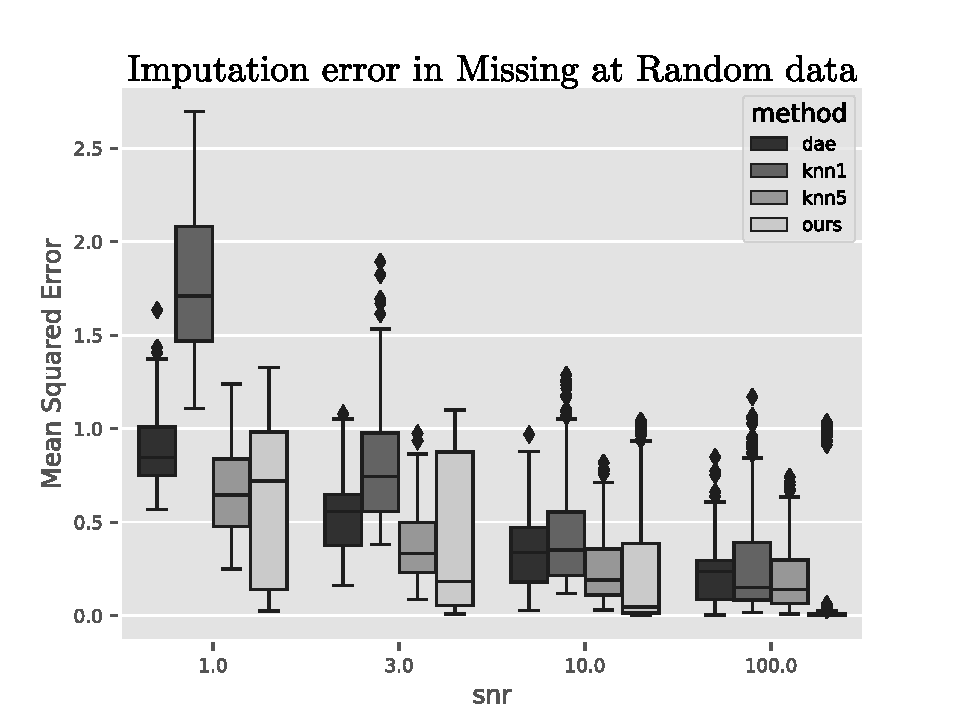
\includegraphics[width=\textwidth]{./tex/fig/mar_imput_err_boxplot.pdf}
        \caption{Missing at random}
        \label{fig:synthetic_benchmark_mar_box}
\end{subfigure}%
\hfill
\begin{subfigure}{.49\textwidth}
	\centering
        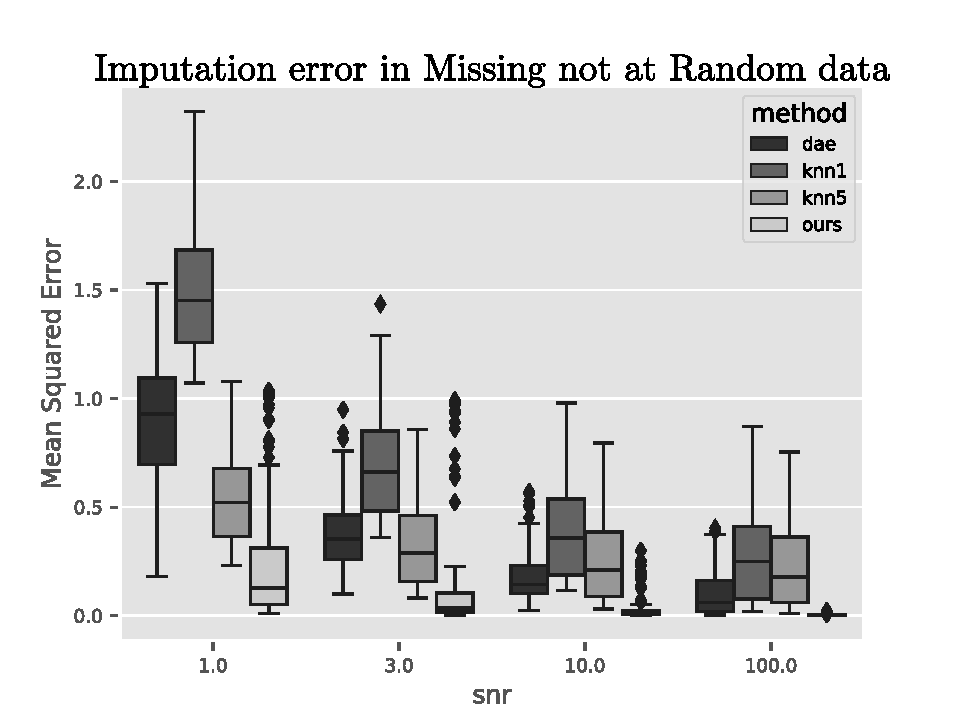
\includegraphics[width=\textwidth]{./tex/fig/mnar_imput_err_boxplot.pdf}
        \caption{Missing not at random}
        \label{fig:synthetic_benchmark_mnar_box}
\end{subfigure}
\caption{
Mean Squared Error of imputation in synthetic datasets. Effect of signal-to-noise ratio (\snr) is shown.
}
\label{fig:synthetic_benchmark_box}
\end{figure}

\begin{figure}[htb]
\centering
\begin{subfigure}{.49\textwidth}
	\centering
        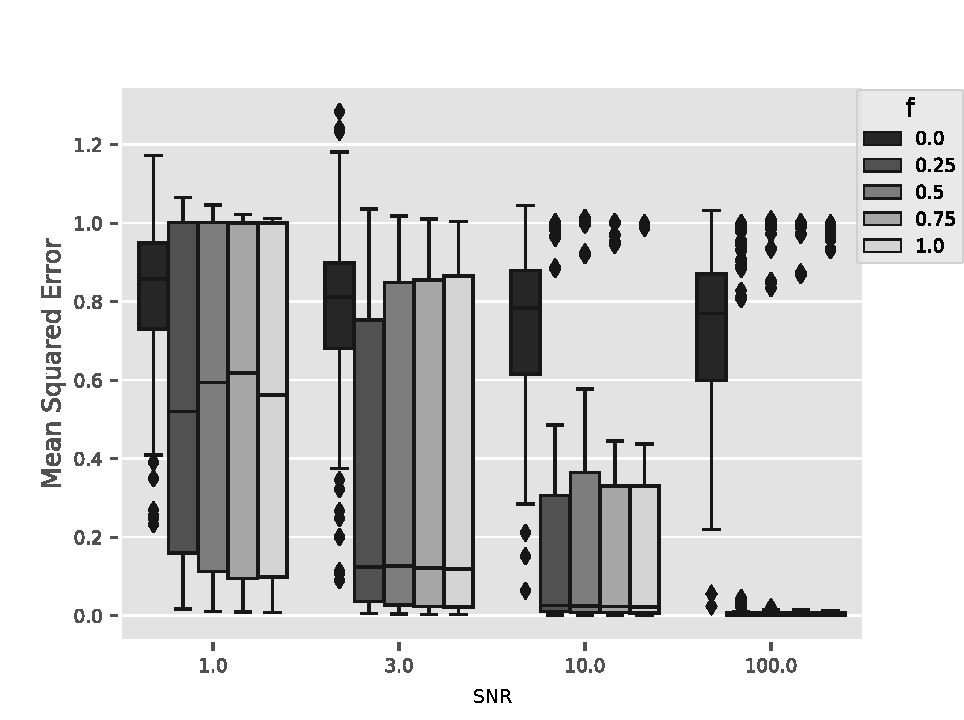
\includegraphics[width=\textwidth]{./tex/fig/mar_pred_err_boxplot.pdf}
        % \caption{Missing at random}
        % \label{fig:synthetic_benchmark_mar_pred_box}
\end{subfigure}%
\caption{
Mean Squared Error of test sets predictions in synthetic datasets.
We show how with already $f \geq 0.25$ (the fraction of observations with all the views) we can significantly reduce the prediction error on testing data-points.
}
\label{fig:synthetic_benchmark_pred_box}
\end{figure}
% \begin{figure}[htb]
% \centering
% \begin{subfigure}{.45\textwidth}
%       \centering
%         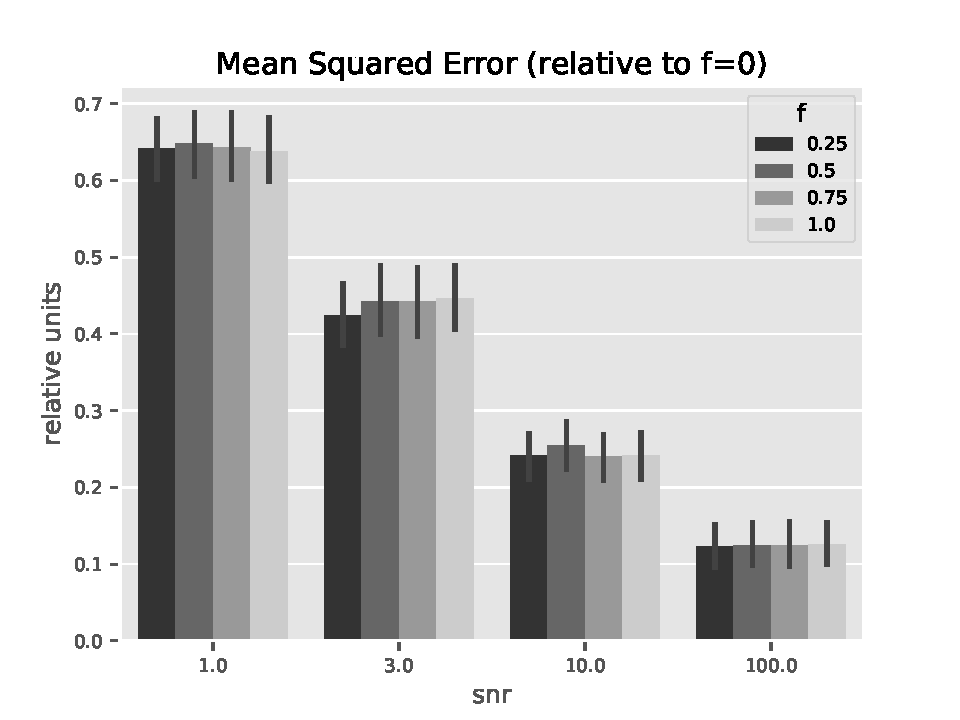
\includegraphics[width=\textwidth]{./tex/fig/mar_barplot.pdf}
%         \caption{Missing at random}
%         \label{fig:synthetic_benchmark_mar_bar}
% \end{subfigure}%
% \hfill
% \begin{subfigure}{.45\textwidth}
%       \centering
%         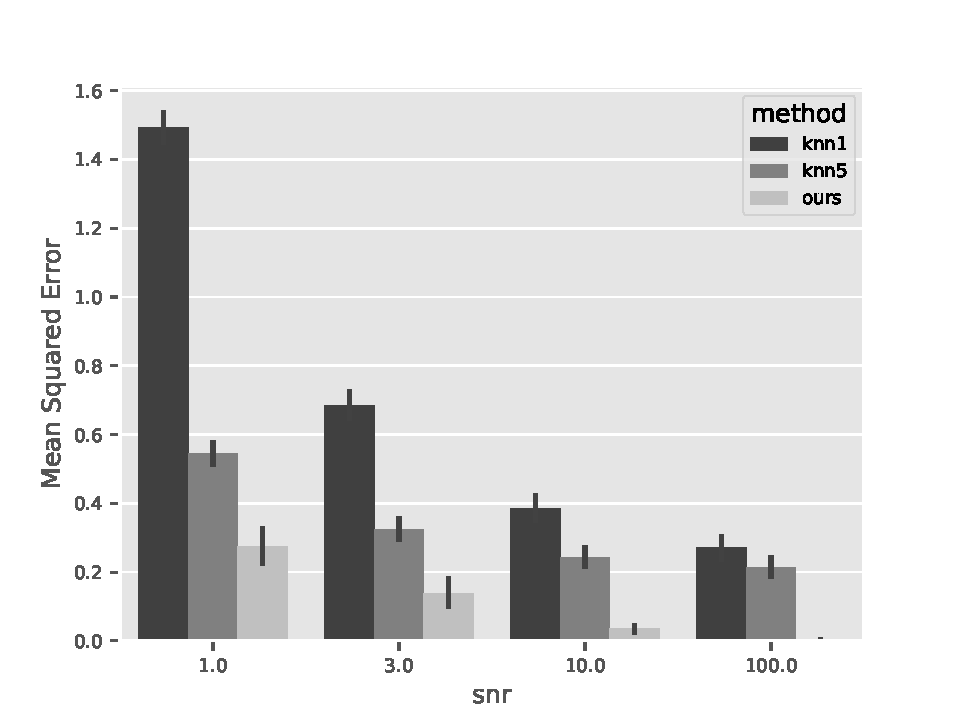
\includegraphics[width=\textwidth]{./tex/fig/mnar_barplot.pdf}
%         \caption{Missing not at random}
%         \label{fig:synthetic_benchmark_mnar_bar}
% \end{subfigure}
% \caption{
% Mean Squared Error of test sets predictions in synthetic datasets. Effect of signal-to-noise ratio (\snr) is shown.
% (a) With $f$ being the fraction of observation with complete views, we show how with already $f \geq 0.25$ we can significantly reduce the prediction error on testing data-points.
% (b) In multi-view datasets where none of the data-point have all the views, and where the available views depends on the specific dataset, we show the prediction performance of our model in comparison with classic k-nearest-neighbors imputation methods.
% }
% \label{fig:synthetic_benchmark_bar}
% \end{figure}



In the synthetic tests our model comes out as the best performer, with a mean MSE improvement compared to best competing method of $17\%$ in MAR cases and $71\%$ in MNAR cases (\figref{fig:synthetic_benchmark_box}).

We notice that DAE is not always better than knn ($k=5$), especially in low \snr\ cases.

We were able to fit the MICE model only on MNAR cases with high \snr\, where it performed poorly (boxplot not shown), while in all the other cases, including all MAR cases, this model did not converge.

In \figref{fig:synthetic_benchmark_pred_box} we show MAR experiments results stratified by \snr\ and by the fraction $f$ of data-points with complete views.
Here we notice how with already $f = 0.25$ we can significantly reduce the prediction error on testing data-points compared to the case $f=0$, where no relationship between views can be established.
Moreover, reaching the ideal case of $f=1$, that is when there are no missing views in the dataset, does not improve significantly the prediction performance of our model.

%%%%%%%%%%%%%%%%%%%%%
%% MEDICAL IMAGING %%
%%%%%%%%%%%%%%%%%%%%%
\section{Experiments on Medical Imaging Datasets}
\label{sec:real}

\begin{table}[!t]
\caption{
Number of subjects per view available in each dataset.
The last columns provide the size of the intersection ($\cap$) and union ($\cup$) of subjects with available views.
The mri from the local dataset is considered as a stand-alone modality as the measures were obtained with a different protocol from the ones in the other datasets.
Notice how in the jont dataset no subject have all the modalities.
}
\centering
\resizebox{\columnwidth}{!}{
\begin{tabular}{lccccc|cc}
\toprule
View:          &  clin &   MRI &  FDG & AV45 &  TAU & $\cap$ & $\cup$ \\
\midrule
Dataset \\
adni1          &   740 &   730 &    - &    - &    - & 730 &  740 \\
adni2          &  1324 &   710 &  424 &  417 &   61 &  53 & 1324 \\
miriad         &    67 &    67 &    - &    - &    - &  67 &   67 \\
oasis3         &   529 &   489 &    - &  148 &    - & 147 &  529 \\
geneva         &   999 &     - &   65 &  120 &   54 &  15 &  999 \\
\midrule
Tot. subjects  &  3659 &  1996 &  489 &  685 &  115 &   0 & 3659 \\
\midrule
Tot. datasets  & 5     & 4     & 2    & 3    & 2    &     &      \\
\bottomrule
\end{tabular}}
\label{table:datasets}
\end{table}

% \begin{table}[!t]
\caption{
Mean Squared Error on unseen test data, $5$-fold cross validation.
Mean (standard deviation) across folds are shown. Best results in boldface.
Test data may belong to the same datset used to train the model (within) or on all the other (cross).
Every modality was predicted from the other available ones.
}
\centering
\begin{tabular}{llcccccc}
\toprule
             &       &         clin &          mri &          fdg &         av45 &          tau &   mri local \\
train & test &              &              &              &              &              &              \\
\midrule
adni1 & within &  0.91 (0.11) &  0.95 (0.13) &            - &            - &            - &            - \\
             & cross &  0.91 (0.29) &  1.01 (0.44) &            - &            - &            - &            - \\
\midrule
adni2 & within &  0.77 (0.11) &  \textbf{0.91} (0.20) &  \textbf{0.82} (0.20) &  \textbf{0.93} (0.22) &  1.20 (0.71) &            - \\
             & cross &  0.82 (0.27) &  1.00 (0.41) &            - &  1.28 (0.46) &  1.67 (1.19) &            - \\
\midrule
miriad & within &  0.74 (0.34) &  1.01 (0.52) &            - &            - &            - &            - \\
             & cross &  0.89 (0.15) &  0.99 (0.18) &            - &            - &            - &            - \\
\midrule
local & within &  0.94 (0.28) &            - &            - &  1.20 (0.28) &  1.43 (1.29) &  \textbf{1.23} (0.35) \\
             & cross &  1.29 (0.28) &            - &            - &  1.13 (0.24) &  \textbf{1.17} (0.75) &            - \\
\midrule
\midrule
average & within &  0.84 (0.21) &  0.96 (0.29) &  \textbf{0.82} (0.20) &  1.06 (0.25) &  1.32 (1.00) &  \textbf{1.23} (0.35) \\
        & cross  &  0.98 (0.25) &  1.00 (0.34) &            - &  1.21 (0.35) &  1.42 (0.97) &            - \\
\midrule
\midrule
% all (dae)        & within &  0.56 (0.05) &  1.02 (0.12) &  0.98 (0.24) &  1.02 (0.17) &  1.11 (0.62) &  1.10 (0.34) \\
% all (knn5)        & within &  \textbf{0.65} (0.04) &  1.03 (0.11) &  1.09 (0.20) &  1.42 (0.17) &  1.29 (0.66) &  \textbf{1.23} (0.38) \\
all       & joint &  \textbf{0.65} (0.05) &  0.95 (0.12) &  0.85 (0.21) &  0.99 (0.20) &  \textbf{1.17} (0.64) &  1.25 (0.35) \\
\bottomrule
\end{tabular}
\label{table:crossvalidation_details}
\end{table}

%\begin{table}[!t]
%\caption{
%Same as above, after average-pooling af means and standard deviations by 
%}
%\centering
%\begin{tabular}{lcccccc}
%\toprule
%{} &         clin &          mri &          fdg &         av45 &          tau &   mri local \\
%train/test   &              &              &              &              &              &              \\
%\midrule
%within &  0.84 (0.21) &  0.96 (0.29) &  0.82 (0.20) &  1.06 (0.25) &  1.32 (1.00) &  1.23 (0.35) \\
%cross  &  0.98 (0.25) &  1.00 (0.34) &            - &  1.21 (0.35) &  1.42 (0.97) &            - \\
%joint  &  0.65 (0.05) &  0.95 (0.12) &  0.85 (0.21) &  0.99 (0.20) &  1.17 (0.64) &  1.25 (0.35) \\
%\bottomrule
%\end{tabular}
%\label{table:crossvalidation}
%\end{table}


% \begin{sidewaystable}
\centering
\begin{tabular}{llllllll}
\toprule
       &      &         clin &           mri &          fdg &         av45 &          tau &   mri\_geneva \\
test dataset & train type &              &               &              &              &              &              \\
\midrule
adni1 & within &  0.90 (0.12) &   0.95 (0.16) &            - &            - &            - &            - \\
       & cross &  1.17 (0.80) &   2.88 (3.10) &            - &            - &            - &            - \\
       & lodo &  0.46 (0.07) &   1.13 (0.16) &            - &            - &            - &            - \\
\midrule
adni2 & within &  0.78 (0.12) &   0.91 (0.24) &  0.85 (0.25) &  0.94 (0.27) &  1.24 (0.93) &            - \\
       & cross &  1.08 (0.64) &   2.17 (2.12) &  4.03 (0.85) &  3.34 (2.65) &  1.33 (0.97) &            - \\
       & lodo &  0.60 (0.29) &   0.81 (0.21) &  3.90 (0.90) &  3.04 (2.52) &  1.10 (0.74) &            - \\
\midrule
miriad & within &  0.76 (0.47) &   1.01 (0.66) &            - &            - &            - &            - \\
       & cross &  7.20 (5.07) &  10.39 (4.47) &            - &            - &            - &            - \\
       & lodo &  2.32 (0.95) &   7.97 (2.14) &            - &            - &            - &            - \\
\midrule
geneva & within &  0.89 (0.33) &             - &  1.15 (0.47) &  1.25 (0.37) &  1.86 (3.04) &  1.20 (0.47) \\
       & cross &  2.69 (1.28) &             - &  6.09 (1.95) &  2.57 (3.04) &  2.36 (2.34) &            - \\
       & lodo &  1.83 (0.90) &             - &  5.99 (1.81) &  1.63 (0.48) &  2.47 (2.51) &            - \\
\midrule
oasis3 & within &  0.71 (0.15) &   0.81 (0.11) &            - &  1.10 (0.42) &            - &            - \\
       & cross &  1.29 (0.74) &   2.43 (2.47) &            - &  1.56 (0.93) &            - &            - \\
       & lodo &  0.76 (0.08) &   0.77 (0.11) &            - &  1.74 (0.34) &            - &            - \\
\bottomrule
       & within &  0.81 (0.24) &  0.92 (0.29) &  1.00 (0.36) &  1.10 (0.35) &  1.55 (1.98) &  1.20 (0.47) \\
       & cross  &  2.69 (1.71) &  4.47 (3.04) &  5.06 (1.40) &  2.49 (2.21) &  1.85 (1.66) &            - \\
       & lodo   &  1.19 (0.46) &  2.67 (0.66) &  4.94 (1.35) &  2.14 (1.11) &  1.79 (1.63) &            - \\
\bottomrule
\end{tabular}
\end{sidewaystable}

\begin{table*}
\centering
\caption{
Mean Squared Error (MSE, the lower the better) measured on test dataset views (clinical scores and imaging derived phenotypes) predicted with our model.
$5$-folds cross-validation results shown as as average (standard deviation).
Models were trained on all the available views in the training dataset, independently of their presence in the testing dataset.
Experiments run in three different conditions depending on the provenance of the training data:
1) `same' dataset as the testing dataset;
2) `different' from the testing dataset (average MSE shown);
3) `leave out test', from all the available datasets except the testing dataset.
By average pooling the results (bottom) we see how in general training on data coming from multiple datasets ameliorates the results.
}
\label{tab:features}
\begin{tabular}{llcccccc}
\toprule
       &      &         clin &           mri &          fdg &         av45 &          tau &   mri local \\
test dataset & train dataset &              &               &              &              &              &              \\
\midrule
adni1  & same           &  0.94 (0.11) &  0.83 (0.10) &            - &            - &            - &            - \\
       & different (avg)    &  0.79 (0.26) &  0.78 (0.14) &            - &            - &            - &            - \\
       & leave out test &  0.47 (0.09) &  0.83 (0.13) &            - &            - &            - &            - \\
\midrule
adni2  & same           &  0.78 (0.16) &  0.68 (0.12) &  0.60 (0.10) &  0.81 (0.12) &  1.29 (0.54) &            - \\
       & different (avg)    &  0.68 (0.29) &  0.73 (0.16) &  1.13 (0.17) &  1.04 (0.27) &  1.10 (0.38) &            - \\
       & leave out test &  0.43 (0.07) &  0.69 (0.11) &  1.14 (0.20) &  0.91 (0.17) &  1.03 (0.37) &            - \\
\midrule
miriad & same           &  2.90 (1.24) &  6.19 (1.52) &            - &            - &            - &            - \\
       & different (avg)    &  5.77 (3.83) &  6.32 (1.54) &            - &            - &            - &            - \\
       & leave out test &  1.91 (1.26) &  5.81 (1.35) &            - &            - &            - &            - \\
\midrule
oasis3 & same           &  0.68 (0.24) &  0.65 (0.12) &            - &  1.30 (0.36) &            - &            - \\
       & different (avg)    &  0.98 (0.40) &  0.79 (0.19) &            - &  1.15 (0.32) &            - &            - \\
       & leave out test &  0.74 (0.10) &  0.78 (0.14) &            - &  1.11 (0.32) &            - &            - \\
\midrule
local  & same           &  1.07 (0.43) &            - &  3.23 (1.01) &  1.70 (0.46) &  1.36 (0.77) &  1.36 (0.36) \\
       & different (avg)    &  2.49 (1.30) &            - &  2.70 (0.76) &  1.52 (0.57) &  1.67 (0.78) &            - \\
       & leave out test &  1.76 (1.09) &            - &  2.71 (0.79) &  1.37 (0.38) &  1.49 (0.69) &            - \\
\midrule
\midrule
average& same           &  1.27 (0.60) &  2.09 (0.77) &  \textbf{1.91} (0.72) &  1.27 (0.34) &  1.32 (0.67) &  1.36 (0.36) \\
       & different (avg)    &  2.14 (1.83) &  2.16 (0.78) &  1.92 (0.55) &  1.24 (0.41) &  1.39 (0.61) &            - \\
       & leave out test &  \textbf{1.06} (0.75) &  \textbf{2.03} (0.69) &  1.92 (0.58) &  \textbf{1.13} (0.30) &  \textbf{1.26} (0.56) &            - \\
\bottomrule
\end{tabular}
\end{table*}

\begin{table}
\centering
\caption{
Experiment of diagnosis classification.
Classification accuracy (the higher the better) from a 5-folds cross-validation experiments is shown.
On average, in-dataset (same) prediction performance is higher with respect to all other cases.
Out-dataset prediction performance is higher if multiple dataset are pooled together (leave out test) with respect to the 
average case where our model is trained with a single dataset (different).
}
\begin{tabular}{llcr}
\toprule
       &      &            \multicolumn{2}{c}{\% accuracy} \\
test dataset & train dataset & mean & std \\
\midrule
adni1  & same            &  61.22 & 5.11 \\
       & different (avg) &  49.43 & 11.56 \\
       & leave out test  &  58.38 & 3.78 \\
\midrule
adni2  & same            &  64.28 & 0.98 \\
       & different (avg) &  46.41 & 5.20 \\
       & leave out test  &  56.95 & 3.11 \\
\midrule
miriad & same            &  90.99 & 8.48 \\
       & different (avg) &  76.45 & 13.07 \\
       & leave out test  &  92.42 & 9.42 \\
\midrule
oasis3 & same            &  80.19 & 4.95 \\
       & different (avg) &  54.34 & 9.32 \\
       & leave out test  &  62.45 & 7.01 \\
\midrule
local  & same            &  76.85 & 4.41 \\
       & different (avg) &  34.12 & 13.13 \\
       & leave out test  &  38.16 & 5.41 \\
\midrule
\midrule
average& same            &  \textbf{74.70} & 4.79 \\
       & different (avg) &  52.15 & 10.46 \\
       & leave out test  &  61.67 & 5.75 \\
\bottomrule
\end{tabular}
\end{table}

\begin{table}[!t]
\caption{
Mean Squared Error (MSE) of test data from adni2.
All models were trained on all the available datasets by holding-out data from the adni2 test dataset.
$5$-folds cross validation of MSE is shown as mean (standard deviation).
Best results in boldface are significant with an $\alpha$ level of 0.01 with respect to both competing methods.
}
\centering
\label{tab:model_comparison}
\begin{tabular}{lccc}
\toprule
View       &          \multicolumn{3}{c}{model}\\
           &          dae &         knn5 &           ours        \\ \cline{2-4}
clin       &  0.73 (0.14) &  0.44 (0.05) &          0.45 (0.07) \\
MRI        &  1.23 (0.31) &  0.88 (0.15) &  \textbf{0.70} (0.13) \\
FDG        &  4.20 (0.56) &  4.15 (0.59) &  \textbf{1.09} (0.15) \\
AV45       &  1.45 (0.35) &  1.20 (0.25) &  \textbf{0.89} (0.15) \\
TAU        &  1.54 (0.82) &  1.44 (0.83) &  \textbf{1.05} (0.45) \\
\bottomrule
\end{tabular}
\end{table}

% \begin{table}[!t]
% \caption{
% Add OASIS3 dataset (clin, mri, av45)
% }
% \centering
% \begin{tabular}{lcccccc}
% \toprule
% model &         clin &          mri & fdg &         av45 &          tau & mri local \\
% % model &              &              &     &              &              &            \\
% \midrule
% knn5              &  0.50 (0.06) &  0.92 (0.13) &   - &  \textbf{1.33} (0.23) &  1.10 (0.54) &  -  \\
% dae               &  0.45 (0.08) &  0.95 (0.15) &   - &  1.49 (0.20) &  1.09 (0.50) &  -  \\
% our               &  \textbf{0.39} (0.05) &  \textbf{0.75} (0.13) &   - &  1.38 (0.21) &  \textbf{0.93} (0.51) &  -  \\
% \bottomrule
% \end{tabular}
% \label{table:model_comparison}
% \end{table}
% 
% \begin{table}[!t]
% \caption{
% Add OASIS3 dataset (clin, mri, av45), ComBat normalize (mri, fdg, av45, tau)
% }
% \centering
% \begin{tabular}{lcccccc}
% \toprule
% model &         clin &          mri & fdg &         av45 &          tau & mri local \\
% % model &              &              &     &              &              &            \\
% \midrule
% knn5              &  0.51 (0.07) &  1.10 (0.17) &   - &  1.16 (0.19) &  \textbf{1.08} (0.62) &  -  \\
% dae               &  0.44 (0.06) &  1.09 (0.17) &   - &  \textbf{1.06} (0.19) &  1.45 (0.70) &  -  \\
% our               &  \textbf{0.42} (0.05) &  \textbf{0.94} (0.15) &   - &  \textbf{1.06} (0.20) &  1.32 (0.71) &  -  \\
% \bottomrule
% \end{tabular}
% \label{table:model_comparison}
% \end{table}
% 
% \begin{table}[!t]
% \caption{
% Add OASIS3 dataset (clin, mri, av45), add Geneva PET, ComBat normalize (mri, fdg, av45, tau)
% }
% \centering
% \begin{tabular}{lcccccc}
% \toprule
% model &         clin &          mri & fdg &         av45 &          tau & mri local \\
% % model &              &              &     &              &              &            \\
% \midrule
% knn5              &  0.50 (0.06) &  1.09 (0.17) &   - &  1.18 (0.20)  &  1.23 (0.92)  &  -  \\
% dae               &  0.42 (0.08) &  1.09 (0.16) &   - &  1.08 (0.19)  &  1.54 (0.87)  &  -  \\
% our               &  \textbf{0.41} (0.06) &  \textbf{0.93} (0.15) &   - &  \textbf{1.07} (0.17)  &  \textbf{1.17} (0.81)  &  -  \\
% \bottomrule
% \end{tabular}
% \label{table:model_comparison}
% \end{table}

% \begin{table}[!t]
\caption{
Mean Squared Error (MSE) of test data from adni2.
All models were trained on all the available datasets by holding-out data from the adni2 test dataset.
$5$-folds cross validation of MSE is shown as mean (standard deviation).
Best results in boldface are significant with an $\alpha$ level of 0.01 with respect to both competing methods.
}
\centering
\label{tab:model_comparison}
\begin{tabular}{lccc}
\toprule
View       &          \multicolumn{3}{c}{model}\\
           &          dae &         knn5 &           ours        \\ \cline{2-4}
clin       &  0.73 (0.14) &  0.44 (0.05) &          0.45 (0.07) \\
MRI        &  1.23 (0.31) &  0.88 (0.15) &  \textbf{0.70} (0.13) \\
FDG        &  4.20 (0.56) &  4.15 (0.59) &  \textbf{1.09} (0.15) \\
AV45       &  1.45 (0.35) &  1.20 (0.25) &  \textbf{0.89} (0.15) \\
TAU        &  1.54 (0.82) &  1.44 (0.83) &  \textbf{1.05} (0.45) \\
\bottomrule
\end{tabular}
\end{table}

% \begin{table}[!t]
% \caption{
% Add OASIS3 dataset (clin, mri, av45)
% }
% \centering
% \begin{tabular}{lcccccc}
% \toprule
% model &         clin &          mri & fdg &         av45 &          tau & mri local \\
% % model &              &              &     &              &              &            \\
% \midrule
% knn5              &  0.50 (0.06) &  0.92 (0.13) &   - &  \textbf{1.33} (0.23) &  1.10 (0.54) &  -  \\
% dae               &  0.45 (0.08) &  0.95 (0.15) &   - &  1.49 (0.20) &  1.09 (0.50) &  -  \\
% our               &  \textbf{0.39} (0.05) &  \textbf{0.75} (0.13) &   - &  1.38 (0.21) &  \textbf{0.93} (0.51) &  -  \\
% \bottomrule
% \end{tabular}
% \label{table:model_comparison}
% \end{table}
% 
% \begin{table}[!t]
% \caption{
% Add OASIS3 dataset (clin, mri, av45), ComBat normalize (mri, fdg, av45, tau)
% }
% \centering
% \begin{tabular}{lcccccc}
% \toprule
% model &         clin &          mri & fdg &         av45 &          tau & mri local \\
% % model &              &              &     &              &              &            \\
% \midrule
% knn5              &  0.51 (0.07) &  1.10 (0.17) &   - &  1.16 (0.19) &  \textbf{1.08} (0.62) &  -  \\
% dae               &  0.44 (0.06) &  1.09 (0.17) &   - &  \textbf{1.06} (0.19) &  1.45 (0.70) &  -  \\
% our               &  \textbf{0.42} (0.05) &  \textbf{0.94} (0.15) &   - &  \textbf{1.06} (0.20) &  1.32 (0.71) &  -  \\
% \bottomrule
% \end{tabular}
% \label{table:model_comparison}
% \end{table}
% 
% \begin{table}[!t]
% \caption{
% Add OASIS3 dataset (clin, mri, av45), add Geneva PET, ComBat normalize (mri, fdg, av45, tau)
% }
% \centering
% \begin{tabular}{lcccccc}
% \toprule
% model &         clin &          mri & fdg &         av45 &          tau & mri local \\
% % model &              &              &     &              &              &            \\
% \midrule
% knn5              &  0.50 (0.06) &  1.09 (0.17) &   - &  1.18 (0.20)  &  1.23 (0.92)  &  -  \\
% dae               &  0.42 (0.08) &  1.09 (0.16) &   - &  1.08 (0.19)  &  1.54 (0.87)  &  -  \\
% our               &  \textbf{0.41} (0.06) &  \textbf{0.93} (0.15) &   - &  \textbf{1.07} (0.17)  &  \textbf{1.17} (0.81)  &  -  \\
% \bottomrule
% \end{tabular}
% \label{table:model_comparison}
% \end{table}


Joint modeling multiple datasets in real scenarios represents an hybrid case between modeling missing at random (MAR) and missing not at random (MNAR) observations, cases which we separately treated in \S\ref{sec:synth}.
Indeed, every dataset may lack of views which are instead present in others by default.
At the same time, in each dataset, there may be missing views for some data-points due to unknown random reasons.
In this section we describe our results on jointly modeling real medical imaging datasets, independently acquired in the context of research studies on human cognitive decline.

\subsection{Data Sources}
Data used in the preparation of this section were obtained from the following sources.
\begin{enumerate}
%
\item From the Alzheimer's Disease Neuroimaging Initiative (ADNI)
\footnote{
\href{http://adni.loni.usc.edu}{adni.loni.usc.edu}.
The ADNI was launched in 2003 as a public-private partnership, led by Principal Investigator Michael W. Weiner, MD. For up-to-date information, see \href{www.adni-info.org}{www.adni-info.org}.
},
a database of brain imaging and related clinical data of cognitively normal subjects and at various stages of cognitive decline.
%
\item From MIRIAD dataset \cite{Miriad}, a database of brain imaging and related clinical data of cognitively normal subjects and data of Alzheimer's.
%
\item From OASIS-3 dataset \citep{oasis3}, a database of brain MRI and PET scans and related clinical data of cognitively normal subjects and subjects at various stages of cognitive decline.
%
\item From a local cohort collected at the University Hospitals, with brain MRI and PET scans and related clinical data of healthy subjects and subjects with various cognitive disorders.
\end{enumerate}
We divided the ADNI dataset into two independent ones:
`adni1', composed by subjects recruited in the initial study,
and `adni2' composed by those subjects subsequently recruited in ADNI-GO, ADNI2, and ADNI3.
Since data modalities and acquisition protocols of `adni1' are different from those of `adni2', we consider these two cohorts as independent datasets.

\subsection{Data Preparation}
All brain MRI scans, except for the ones in the local cohort, were processed with FreeSurfer \footnote{\href{https://surfer.nmr.mgh.harvard.edu/}{surfer.nmr.mgh.harvard.edu}} \citep{freesurfer} to measure brain cortical and sub-cortical volumes.
We took measures on regions defined in the Desikan-Killiany atlas \cite{Desikan2006}.
MRIs in the local cohort were processed with SPM \cite{Ashburner2000} to measure gray matter density in the brain.



 images were processed with SPM
\subsection{Views}
From the five datasets (`adni1', `adni2', `miriad', `oasis3', `local') we grouped the observations into the following views.
1) `clin': grouping age and the Mini-Mental cognitive score (MMSE).
2) `mri': grouping brain volumes computed with FreeSurfer \footnote{
\href{https://surfer.nmr.mgh.harvard.edu/}{surfer.nmr.mgh.harvard.edu}
}.
3) `fdg': average brain glucose uptake measured through the analysis of FDG-PET scans.
4) `av45': average brain amyloid uptake measured through the analysis of AV45-PET scans.
5) `tau': average brain protein Tau uptake measured through the analysis of TAU-PET scans.
6) `mri local': this is a view only present in the `local' dataset, composed by measurements on brain gray matter density derived from SPM \cite{Ashburner2000}.

All the imaging measurements are averaged on the regions of interests defined in the Desikan-Killiany atlas \cite{Desikan2006}
In \tabref{table:datasets} we show the number of observations stratified by dataset and modality.
Please note that the only view in common across datasets is the clinical one, composed by MMSE and age features only.

\subsection{Fitting procedure}
For the model architecture, we choose the likelihood function as in \eqnref{eq:decoder}.
We then choose to parametrize the encoder as:
\begin{equation}
\label{eq:dropout_posterior}
    q_{d,n,w}(\z) = \Gauss{\mub = \mathbf{V}_w^{(\mu)} \xdnw}{\Sigmab = \text{diag}(\sqrt{\alphab} \odot \mub)^2}.
\end{equation}
The posterior distribution so defined is known as \textit{dropout posterior}.
The dropout parameter $\alphab$ has components $\alpha_i = \nicefrac{p_i}{1-p_i}$ linked to the probability $p_i$ of dropping out the $i$-th latent variable component \cite{Wang2013}.
It has been shown that the association of this dropout posterior with a log-uniform prior distribution $\pz$ leads to sparse and interpretable models \cite{Antelmi2019,Molchanov2017}.

We fit our multi-view model one dataset at a time, and lastly on the whole dataset pool.
We will refer to this last model as `all'.
Observations were divided into five splits, stratified to keep an intra-dataset proportion of views as close as possible as the ones of the original datasets.
After setting a dropout threshold to $0.5$ we measured, through the mean squared error, the prediction error of the dataset-specific models on the testing hold-out observations of the same dataset (within).
To have a measure of the generalization ability for each model, we measured the prediction accuracy also on all the test sets not belonging to the same dataset of the trainig set (cross).
The same was done with the model `all'.
In this case the hold out observations belong to the whole dataset pool and we will refer to its testing set as the `joint' set.

\subsection{Results}
In \tabref{tab:features} we show for each trained multi-view model, the prediction error on the within-dataset test sets, cross-dataset test sets, and joint set, whenever computable.
We notice that the generalization performance of the model `all' is almost always the best in predicting the `clin' and `mri' views.
These are also the views most represented in all the datasets.
We also note that joint model systematically outperforms the dataset-specific models when applyed across dataset.
Moreover it generally provides better predictions even respect to the within-dataset results.
On the other extreme, views belonging only to a specific dataset, such as `fdg' in `adni2' and `mri local' in the `local' dataset are better predicted with dataset-specific models.
In the remainig cases of `av45' and `tau', the joint model seems, on average, to perform better than the single dataset-specific ones.


\section{Discussion}

In both the experiments on synthetic and real data, our model compared favorably with respect to state of the art benchmark methods.

An interesting result is the one presented in \figref{fig:synthetic_benchmark_pred_box}, suggesting that collecting a minimum amount of data-points with complete views is enough for our model to capture the joint relationship among views.
The empirical bound on this minimum level of data-points with all available views amounts to $25\%$.
In fact, in our synthetic tests, training on scenarios with completeness level above this bound does not seem to improve significantly the testing results.
This condition may be explained by the high collinearity between features due to the linear mappings used to generate the multi-view data.
The same bound may be noticed also in our showcase experiment (\S~\ref{sec:proof_of_concept}) where we jointly modeled MRI and FDG-PET brain images.
This results suggest that our model can reach its highest prediction power also when data collection resources are scarce,
such as in studies were the acquisition of complete observations is hampered by economical reasons or subject dropout.
% This condition may be due to overtraining, where collecting more data may not necessary to improve the model performance \citep{Bilbao2017}.
% We think that this fact can have a positive impact in studies were the acquisition of complete observations is hampered by economical or ethical reasons.

\textcolor{blue}{
\refnum{\#23}
	As a secondary result, we report the positive performance of knn (k = 5) in synthetic scenarios, especially in low snr cases, and on real data experiment, were it is most of the time superior to the DAE.
	This finding is corroborated by \cite{Platias2020} were knn is found to be superior to methods based on autoencoders.
}

\textcolor{blue}{
\refnum{\#24, \#25}
	The experimental results on real medical imaging datasets (\tabref{tab:features}, \tabref{tab:classifier}) show on the horizontal axes the clear improvement of our MT-MCVAE method with respect to the MCVAE, that inspired our work,
	given the very same training and testing conditions for both of models.
	The features and diagnosis prediction clearly improves when using our method, that allows to not discard observations with missing views in the training phase.
	On the same tables, when read on the vertical axes, we note that models trained and tested on the same single dataset (STIB cases) tend to be more accurate than those trained on multiple other datasets (STEB cases).
	As this usually happens when the problem of domain shift is such that observations coming from different datasets are not identically distributed,
	we want to emphasize that we mitigated this problem with a data harmonization step based on ComBat \citep{combat},
	one of the state-of-the-art normalization method in biomedical applications \citep{Fortin2017, Fortin2018, Orlhac2020}.
	For this reason, we believe that the domain shift has a marginal impact for the application proposed in our study,
	and that those differences on the vertical axes are most likely due to the large variety of number of observations, available views, and differences in stratification by diseases in the datasets (\cf \tabref{table:datasets}, \tabref{tab:dx_stratification}).
}

In feature prediction experiments (\tabref{tab:features_mtl}) we showed that MT-MCVAE models trained jointly on multiple neuroimaging datasets (ADNI, MIRIAD, OASIS-3, Geneva cohort)
perform generally better than the ones trained on a single dataset.
We suspect that there are two reasons explaining these results.
The first is that modeling simultaneously multiple datasets with our method brings more variability and information at play, making the generalization to unseen data less prone to prediction errors.
The second reason maybe that every decoder, associated to its specific view, acts, through the shared latent space, as a regularizer for all the other decoders.

In experiments where we seek to classify subjects to predict their cognitive status (\tabref{tab:classifier_mtl}),
the MT-MCVAE generalizes better to new unseen datasets when trained jointly on multiple datasets (MTL cases) with respect to cases where the training happens on a single dataset.
We notice that the best results happen in cases where testing data and training data come from the same dataset (ST cases), that is when the testing dataset is not anymore unseen to our model.
This is a different result than the analogous one in the feature prediction experiments, and we argue that the reason may be due to the lack of the regularization mechanism induced by having concurring decoders.
Indeed, the MT-MCVAE classifier is composed by a single decoder only, which can become highly specialized in decoding testing data coming from the same dataset of the training data.

In our non linear experiments we did not capture any improvement by using deep architectures with respect to simple linear mappings,
in both feature prediction \tabrefp{tab:features_mtl_nl} and classification tasks \tabrefp{tab:classifier_mtl_nl} on real neuroimaging datasets.
These results are in line with our previous work \citep{Antelmi2019}, were we benchmarked other auto-encoding based methods on observations coming from the ADNI dataset.
We suspect that this result is due to the general high heterogeneity and relatively small sample size of typical neuroimaging data.
\textcolor{blue}{
	\refnum{\#11}
	We also report no significant differences between the EmbraceNet and our MT-MCVAE \tabrefp{tab:classifier_mtl_nl},
	although we note that is only with the latter that we have a framework adaptable to both classification and modality-to-modality prediction tasks.
}

In our work we have thoroughly investigated architectures with a one-to-one correspondence between encoding and decoding views.
This makes our model part of the family of the auto-encoders, where the model acts as identity transformation between the input and the output.
Other architectures are nevertheless possible, such as the classifier described in \S~\ref{ssec:classifier}
In general, there may be an $m$-to-$n$ relationship, with partially overlapping views among $m$ input views and $n$ output views.
Investigating the properties of all the possible architectures is beyond the scope of this work.

\textcolor{blue}{
\refnum{\#24}
	As final remark, we want to stress that our model is based on the assumption of independent and identical distributed observations.
	This assumption may be limiting in healthcare datasets, such as the ones used in this work.
	In our work we mitigated these biases by harmonizing the datasets before applying our model, and we leave the extension and development of a bias-transparent multi-view models to future works.
}

\section{Conclusions}
We proposed a new multi-task latent variable generative model able to learn simultaneously from multiple datasets, even in the presence of non-overlapping views among all the datasets.
The available overlap between pairs of datasets allows the information to flow through all the views in the dataset pool.
Since the learned view-specific parameters are shared among datasets, missing views can be automatically imputed for every dataset.
The method proposed in this work is a coherent extension of classical variational generative models, making the training fast and scalable.
Being dataset agnostic, our method allows to integrate all the available data into a joint model, gathering  all the available information from multiple datasets at the same time.
We conducted extensive tests for the joint modeling of synthetically generated data and of multi-modal neuroimaging datasets from independent dementia studies and associated clinical data, showing the competitiveness of our method with respect to the state of the art.
Thanks to its general formulation, the proposed method can find applications beyond the neuroimaging research field.

\subsection*{Acknowledgments}
\label{sec:ack}

This work has been supported by:
\begin{itemize}
\item the French government, through the UCAJEDI Investments in the Future project managed by the National Research Agency (ANR) with the reference number ANR-15-IDEX-01;
\item the French government, through the 3IA Côte d'Azur Investments in the Future project managed by the National Research Agency (ANR) with the reference number ANR-19-P3IA-0002;
\item the grant AAP Santé 06 2017-260 DGA-DSH, and by the Inria Sophia Antipolis - Méditerranée, "NEF" computation cluster.
\item Data collection and sharing for this project was funded by the Alzheimer's Disease Neuroimaging Initiative (ADNI) (National Institutes of Health Grant U01 AG024904) and DOD ADNI (Department of Defense award number W81XWH-12-2-0012).
ADNI is funded by the National Institute on Aging, the National Institute of Biomedical Imaging and Bioengineering, and through generous contributions from the following: AbbVie, Alzheimer's Association; Alzheimer's Drug Discovery Foundation; Araclon Biotech; BioClinica, Inc.; Biogen; Bristol-Myers Squibb Company; CereSpir, Inc.; Cogstate; Eisai Inc.; Elan Pharmaceuticals, Inc.; Eli Lilly and Company; EuroImmun; F. Hoffmann-La Roche Ltd and its affiliated company Genentech, Inc.; Fujirebio; GE Healthcare; IXICO Ltd.; Janssen Alzheimer Immunotherapy Research \& Development, LLC.; Johnson \& Johnson Pharmaceutical Research \& Development LLC.; Lumosity; Lundbeck; Merck \& Co., Inc.; Meso Scale Diagnostics, LLC.; NeuroRx Research; Neurotrack Technologies; Novartis Pharmaceuticals Corporation; Pfizer Inc.; Piramal Imaging; Servier; Takeda Pharmaceutical Company; and Transition Therapeutics.
The Canadian Institutes of Health Research is providing funds to support ADNI clinical sites in Canada.
Private sector contributions are facilitated by the Foundation for the National Institutes of Health (\url{www.fnih.org}).
The grantee organization is the Northern California Institute for Research and Education, and the study is coordinated by the Alzheimer's Therapeutic Research Institute at the University of Southern California.
ADNI data are disseminated by the Laboratory for NeuroImaging at the University of Southern California.
\item Data used in the preparation of this article were obtained also from the MIRIAD database.
The MIRIAD investigators did not participate in analysis or writing of this report.
The MIRIAD dataset is made available through the support of the UK Alzheimer's Society (Grant RF116).
The original data collection was funded through an unrestricted educational grant from GlaxoSmithKline (Grant 6GKC).
\item Data were also provided by OASIS-3 \citep{oasis3}: Principal Investigators: T. Benzinger, D. Marcus, J. Morris; NIH P50AG00561, P30NS09857781, P01AG026276, P01AG003991, R01AG043434, UL1TR000448, R01EB009352. AV-45 doses were provided by Avid Radiopharmaceuticals, a wholly owned subsidiary of Eli Lilly.
\end{itemize}


%% The Appendices part is started with the command \appendix;
%% appendix sections are then done as normal sections
%% \appendix

%% \section{}
%% \label{}

%% If you have bibdatabase file and want bibtex to generate the
%% bibitems, please use
%%
\bibliographystyle{elsarticle-harv} 
\bibliography{./tex/biblio}

%% else use the following coding to input the bibitems directly in the
%% TeX file.

% \begin{thebibliography}{00}
% 
% %% \bibitem[Author(year)]{label}
% %% Text of bibliographic item
% 
% \bibitem[ ()]{}
% 
% \end{thebibliography}
\end{document}

\endinput
%%
%% End of file `elsarticle-template-harv.tex'.
